\chapter{Pianificazione}
Lo sviluppo del\glossario{progetto}è diviso in cinque periodi:
\begin{itemize}
    \item \textbf{Analisi} (AN);
    \item \textbf{Revisione Analisi} (RA);
    \item \textbf{Progettazione della base tecnologica} (PT);
    \item \textbf{Progettazione di Dettaglio e Codifica} (PDC);
    \item \textbf{Validazione} (VV).
\end{itemize}
In ogni periodo sono presenti delle attività da svolgere, alle quali sono associate una o più risorse. Ogni attività è sottoposta a\glossario{verifica}, per semplificare il processo di Validazione. Il \textit{Responsabile} è tenuto a rendere più dettagliata la pianificazione delle attività.\\
Le attività sono suddivise in più sotto-attività.\\
Nel\glossario{Gantt}vengono riportate:
\begin{itemize}
    \item \textbf{Attività:} contengono più sotto-attività. Nel Gantt sono rappresentate con una linea grigia;
    \item \textbf{Milestone$_{G}$:} rappresenta la data ultima prevista per il completamento di un insieme prestabilito di attività. Ha durata di 0 (zero) giorni e coincide con la data della successiva revisione o l'approvazione complessiva di tali attività. È rappresentata nel Gantt con un rombo giallo;
    \item \textbf{Sotto-attività:} attività atomiche che possono essere svolte da una persona. Nel Gantt sono rappresentate con una linea blu.  
\end{itemize}
\section{Analisi}
\textbf{Periodo:} da 2018-11-16 a 2019-01-14\\L'Analisi inizia in concomitanza con la pubblicazione dei\glossario{capitolati}d’appalto e termina alla prima settimana della  Revisione dei Requisiti (RR).\\
Le attività della fase di Analisi sono:
\begin{itemize}
    \item \textbf{Studio di Fattibilità:} vengono valutati tutti i capitolati d'appalto. La valutazione è basata sull'interesse personale di ogni membro del gruppo, sulla complessità prevista e sui rischi che possono emergere. Viene data anche una descrizione generale del capitolato e una analisi preliminare.\\Viene svolta come prima attività, in quanto ritenuta bloccante per l'\textit{Analisi dei requisiti};
    \item \textbf{Norme di Progetto:} le \textit{Norme di Progetto} contengono le regole che il gruppo dovrà seguire durante l'attuazione di tutte le attività. I verificatori certificheranno il rispetto delle norme;
    \item \textbf{Analisi dei Requisiti:} l'analisi preliminare nello Studio di Fattibilità viene approfondita;
    \item \textbf{Piano di Progetto:} Il textit{Responsabile} redige il \textit{Piano di Progetto}, rispettando i vincoli posti dalla \glossario{proponente}.\\Questo documento ha l'obiettivo di regolare le attività svolte dal gruppo;
    \item \textbf{Piano di Qualifica:} Il \textit{Piano di Qualifica} contiene le strategie utili al raggiungimento degli obiettivi della \glossario{proponente}, del gruppo e inerenti alla qualità dei processi di sviluppo.\\L'obiettivo è quello di rendere la qualità quantificabile e misurabile;
    \item \textbf{Glossario:} scritto in modo incrementale, contiene la spiegazione dei termini più tecnici utilizzati nei documenti. Questa attività è svolta da tutti i membri del gruppo, in parallelo con la redazione di tutti i documenti;
    \item \textbf{Lettera di presentazione:} documento presentato al committente che permette al gruppo di partecipare alla gara d’appalto per il capitolato$_{G}$.
\end{itemize}
I ruoli maggiormente coinvolti sono: \textit{Responsabile}, \textit{Amministratore} e \textit{Analista}.
\begin{figure} [h]
    \centering
    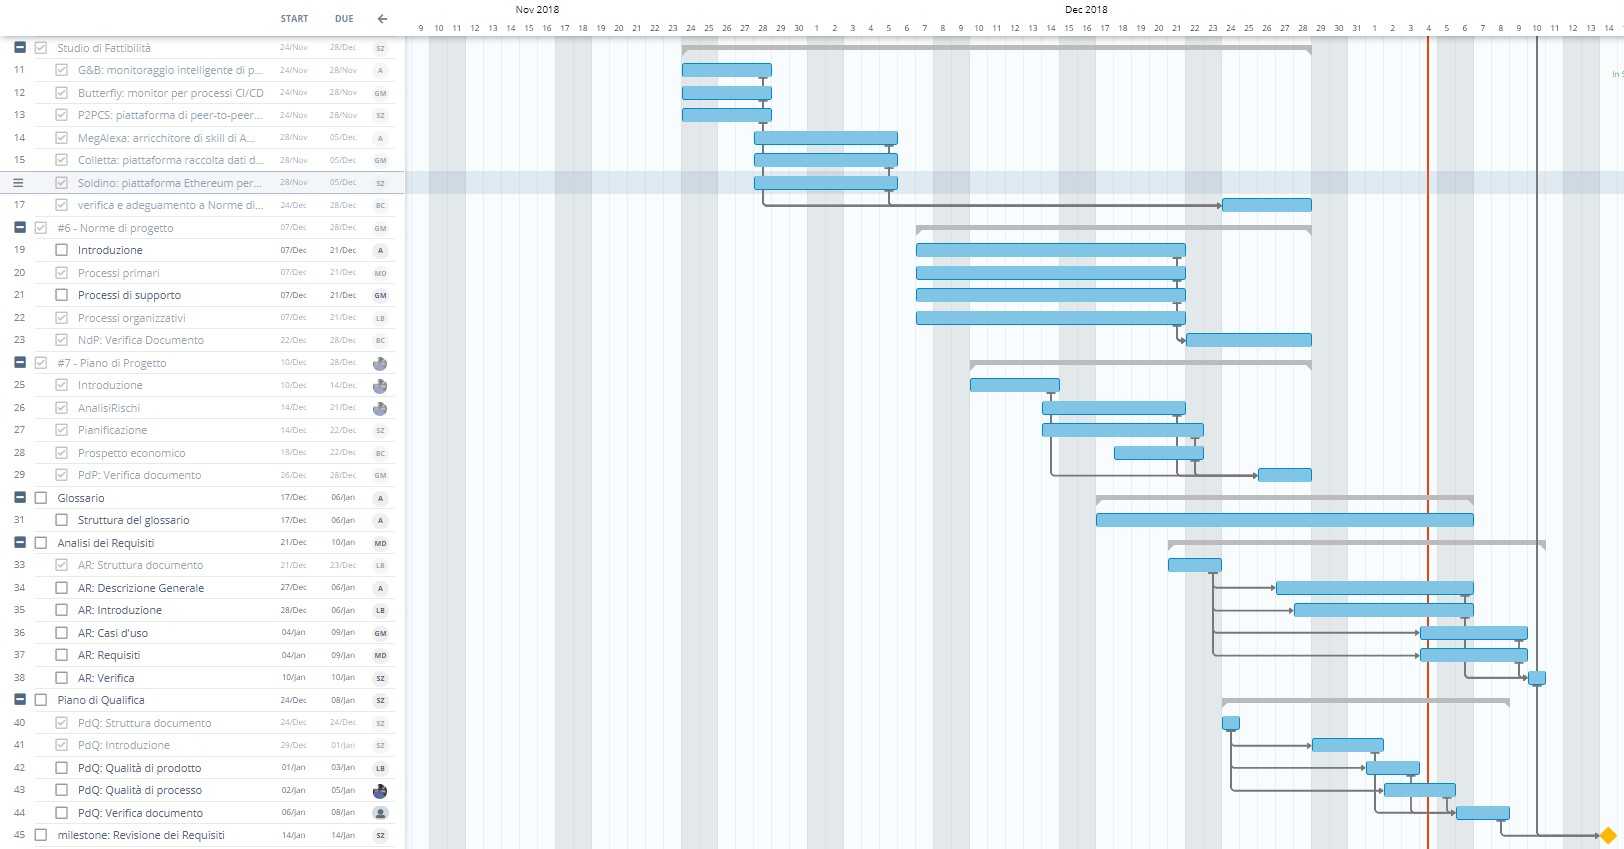
\includegraphics[scale=0.3]{./images/analisi.jpg}
    \caption{\textit{Diagramma di}\glossario{Gantt}: Analisi }\label{}
\end{figure}
\section{Revisione Analisi}
\textbf{Periodo:} da 2019-01-21 a 2019-02-07\\
La Revisione Analisi inizia dopo la Revisione dei Requisiti e termina con l’inizio della Progettazione della base tecnologica. Questo periodo viene utilizzato dal team per consolidare i requisiti richiesti dal sistema e per migliorare i documenti già redatti.\\
Le attività della fase di Revisione Analisi sono:
\begin{itemize}
    \item \textbf{Incremento e Verifica$_{G}$:} tutti i documenti vengono aggiornati in base ai risultati della Revisione dei Requisiti;
    \item \textbf{Glossario:} questa attività consiste nel miglioramento del \textit{Glossario}.
\end{itemize}
I ruoli maggiormente coinvolti sono: Responsabile, Verificatore e Analista.
\begin{figure} [h]
    \centering
    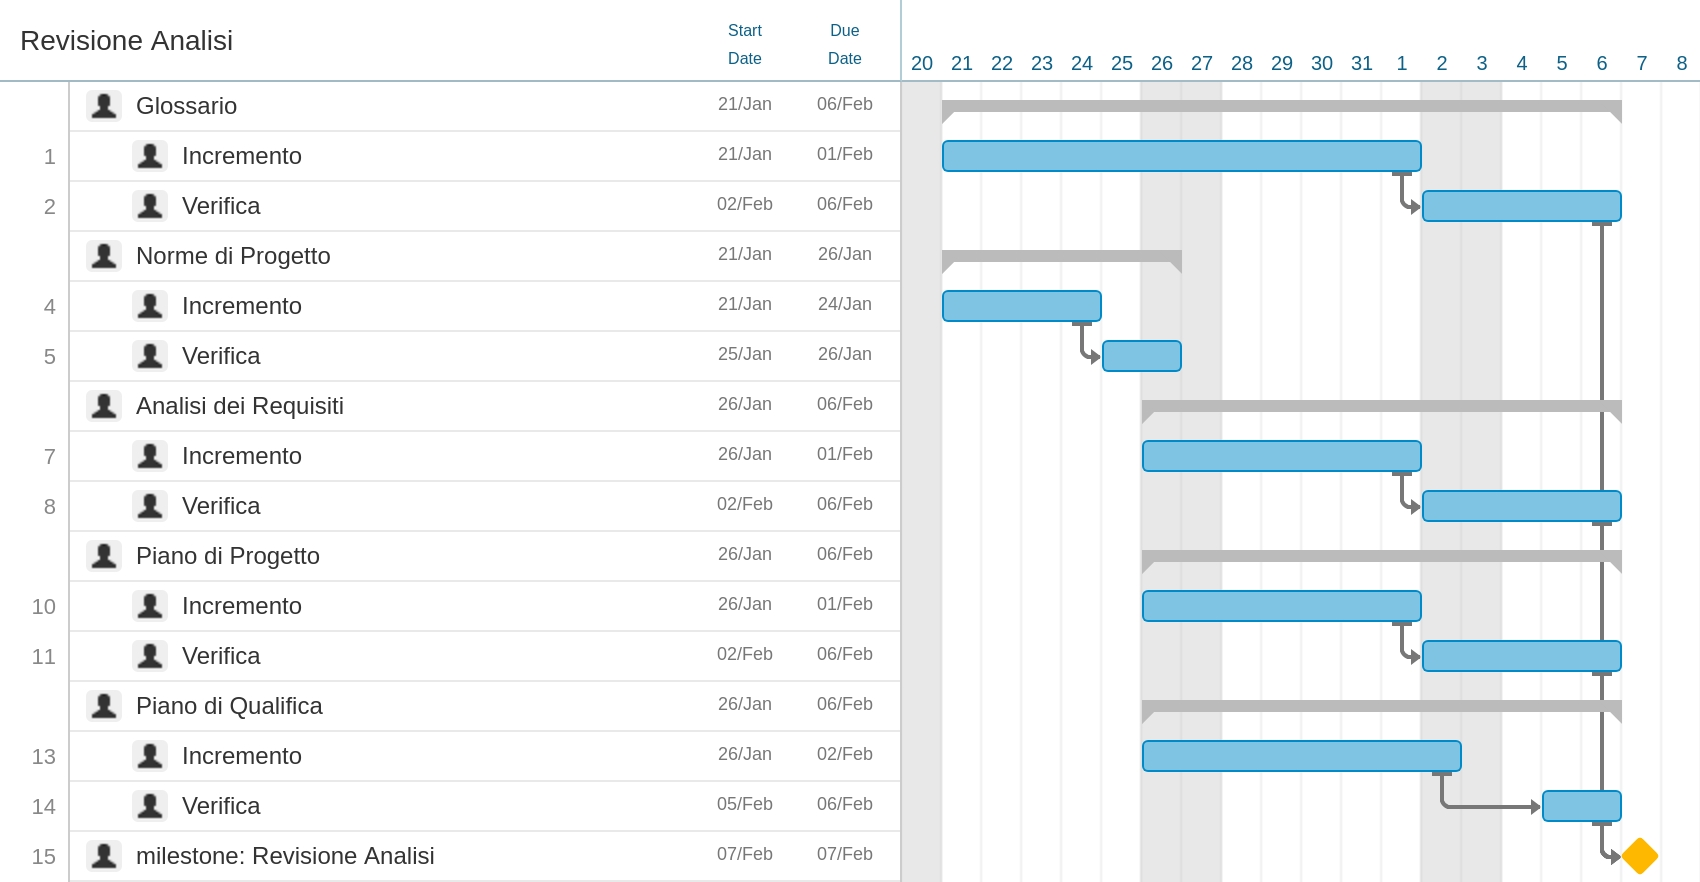
\includegraphics[scale=0.2]{./images/revisione_analisi.jpg}
    \caption{Diagramma di Gantt: Revisione Analisi }\label{}
\end{figure}
\newpage
\section{Progettazione della base tecnologica}
\textbf{Periodo:} da 2019-02-07 a 2019-03-08\\
La Progettazione della base tecnologica inizia al termine della Revisione Analisi e termina con la consegna del\glossario{prodotto}alla Revisione di Progettazione.\\
Le attività della fase di Progettazione della base tecnologica sono:
\begin{itemize}
    \item\textbf{Technology baseline}: in questa attività vengono studiate e analizzate le tecnologie, i framework e le librerie per lo sviluppo del \glossario{Proof of Concept}. Questa attività è considerata critica e bloccante per la prosecuzione del progetto.
    Il prodotto di questa attività viene presentato in una discussione con modalità \glossary{Agile};
    \item \textbf{Incremento e Verifica$_{G}$}: tutti i documenti vengono aggiornati;
    \item \textbf{Glossario}: questa attività consiste nel miglioramento del \textit{Glossario}.
\end{itemize}
I ruoli maggiormente coinvolti sono: \textit{Responsabile}, \textit{Amministratore}, \textit{Progettista}, \textit{Programmatore}, \textit{Verificatore} e \textit{Analista}.
\begin{figure} [h]
    \centering
    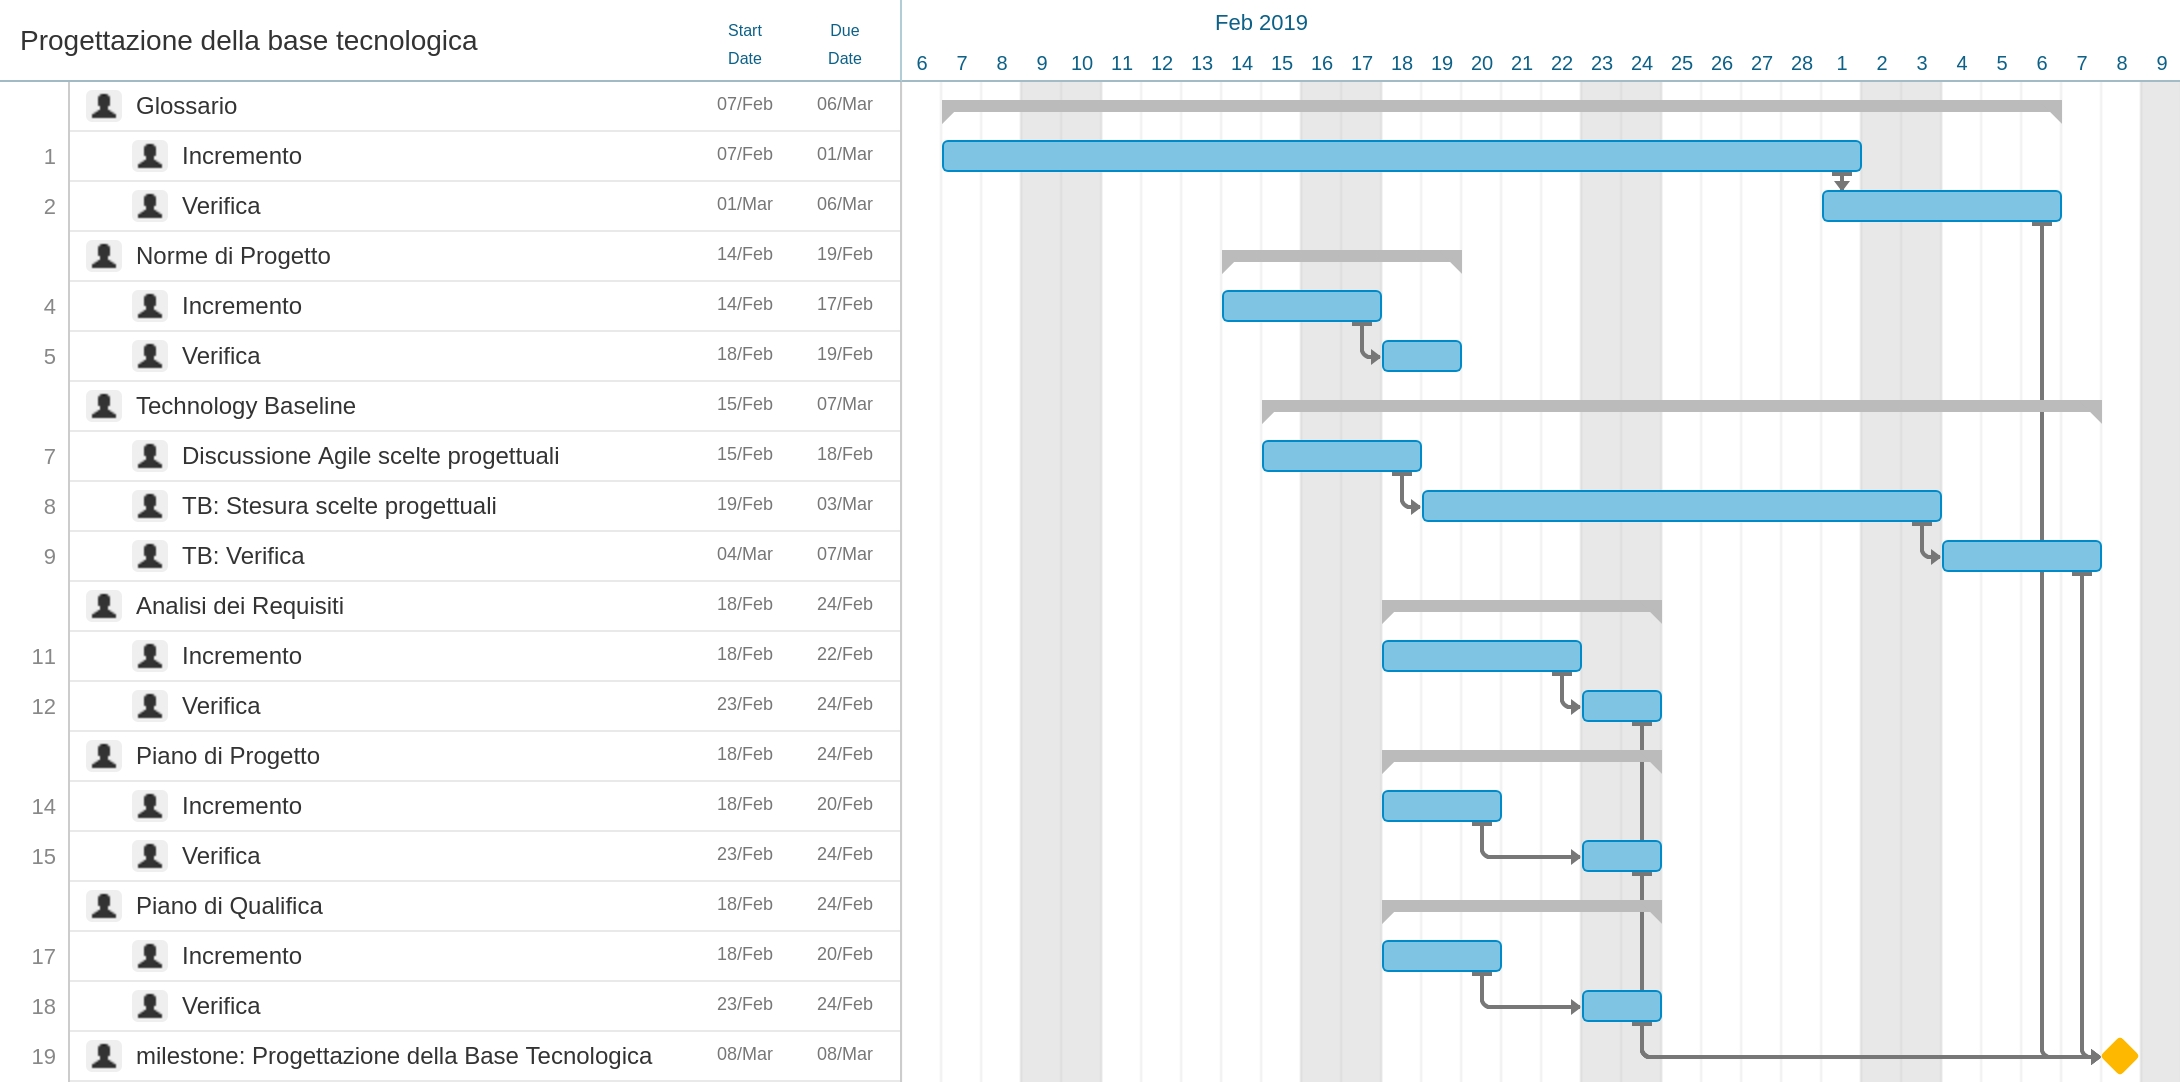
\includegraphics[scale=0.13]{./images/base_tecnologica.jpg}
    \caption{\textit{Diagramma di}\glossario{Gantt}: Base tecnologica }\label{}
\end{figure}
\newpage
\section{Progettazione di Dettaglio e Codifica}
\textbf{Periodo:} da 2019-03-08 a 2019-04-12\\
Questo periodo inizia dopo la Revisione di Progettazione e termina  alla Revisione di Qualifica.\\Le attività della fase di Progettazione di Dettaglio e Codifica sono:
\begin{itemize}
	\item \textbf{Product baseline}: questa attività presenta i diagrammi delle classi e di sequenza coerentemente con quando indicato nella Technology baseline; 
    \item \textbf{Codifica:} i programmatori sviluppano secondo quanto indicato nelle fasi di progettazione;
    \item \textbf{Incremento e Verifica$_{G}$:} tutti i documenti vengono aggiornati in base al risultato della Revisione di Progettazione;
    \item \textbf{Glossario:} questa attività consiste nel miglioramento del \textit{Glossario}.
    \item \textbf{Manuali}: manuali utente e sviluppatore;
\end{itemize}
I ruoli maggiormente coinvolti sono: \textit{Responsabile}, \textit{Amministratore}, \textit{Progettista}, \textit{Verificatore} e \textit{Programmatore}.
\begin{figure} [h]
    \centering
    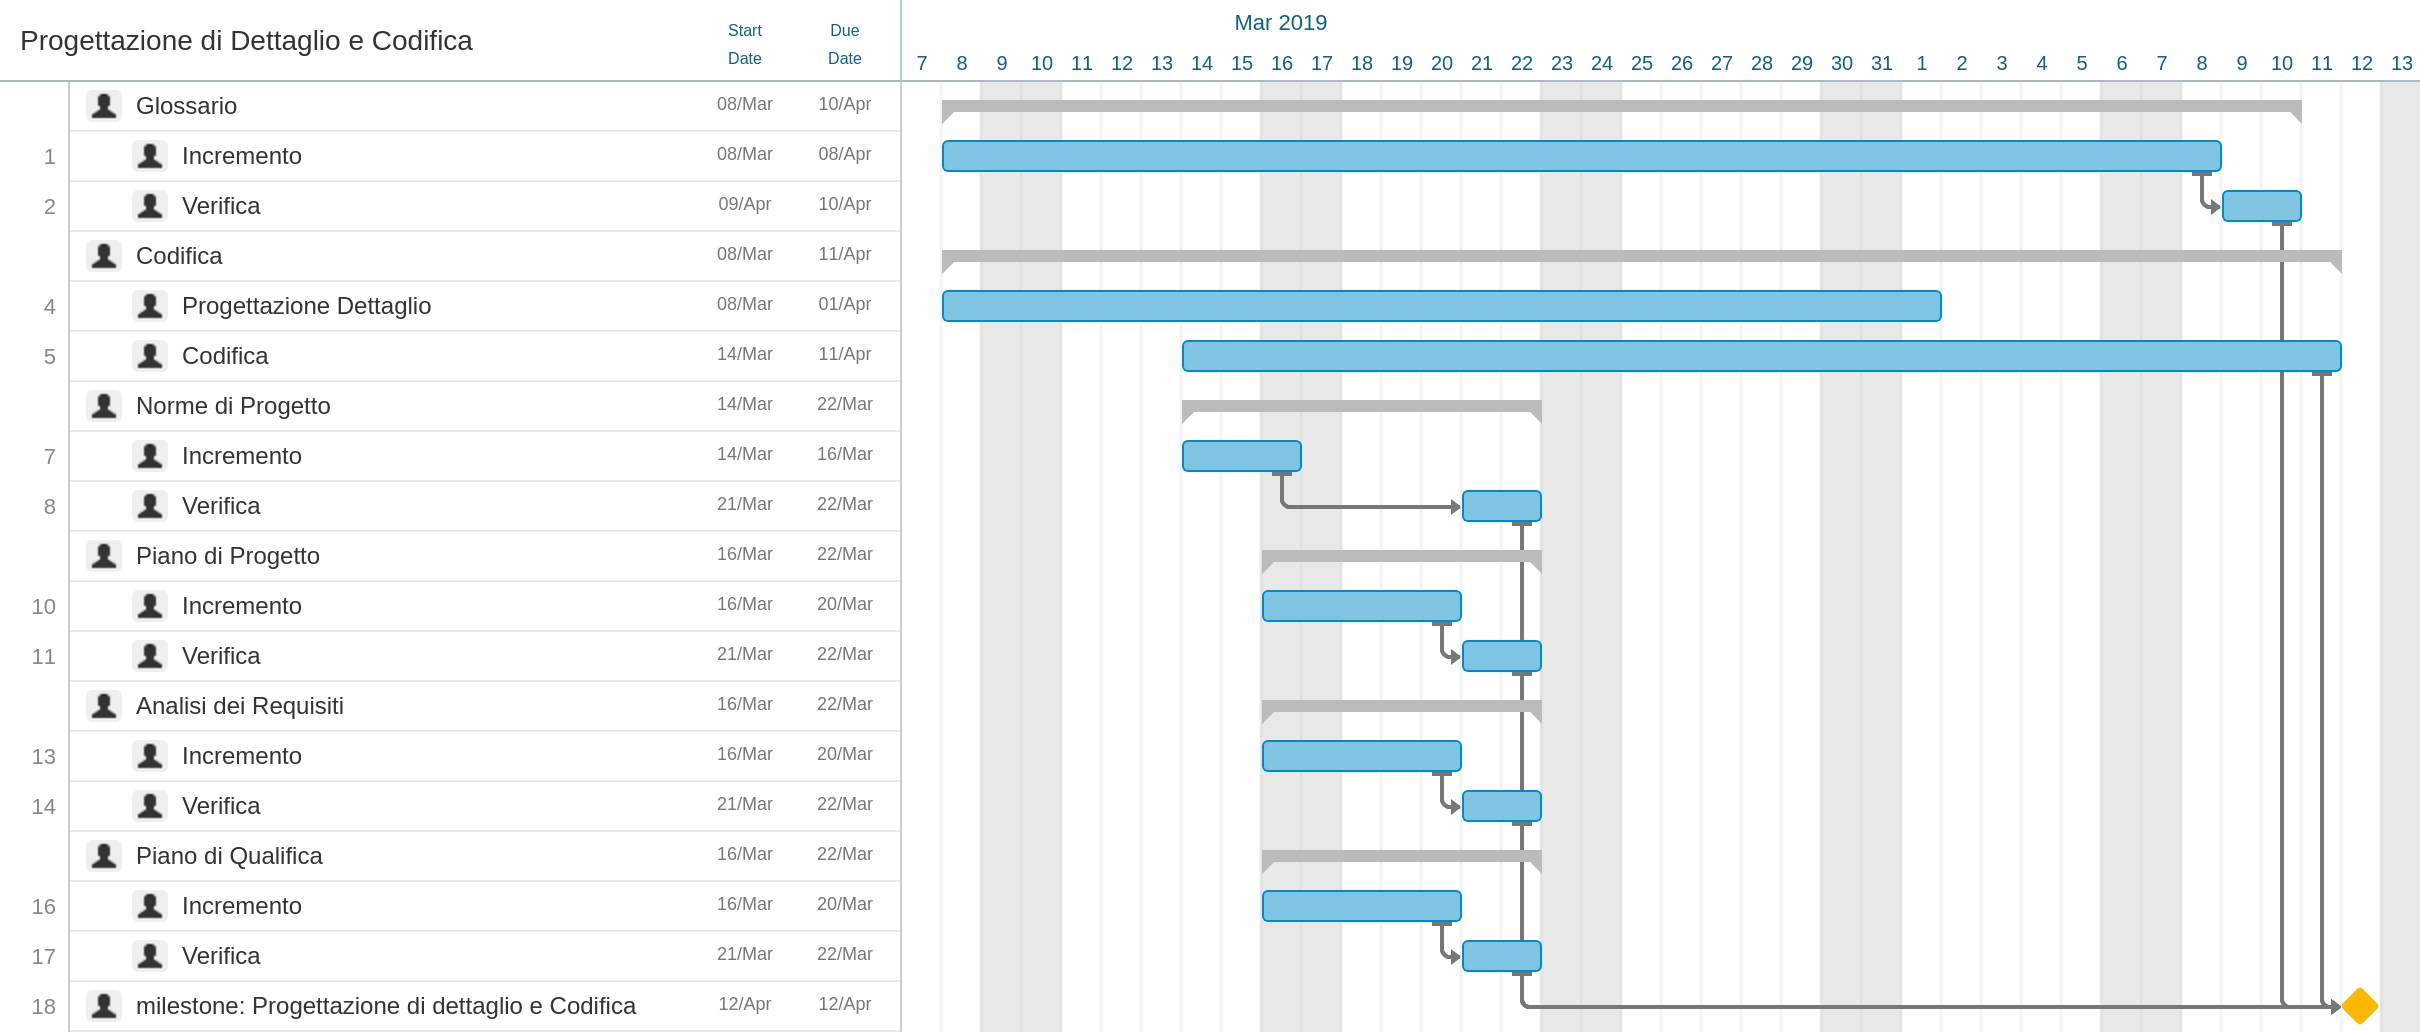
\includegraphics[scale=0.14]{./images/codifica.jpg}
    \caption{\textit{Diagramma di}\glossario{Gantt}: Progettazione di dettaglio e Codifica }\label{}
\end{figure}
\newpage
\section{Validazione e Collaudo}
\textbf{Periodo:} da 2019-04-12 2019-05-17\\
Questo periodo inizia al termine della Progettazione di Dettaglio e Codifica e si conclude con la Revisione di Accettazione.\\Con la Validazione il team svolge le ultime attività di Verifica e prepara il sistema per la Validazione e il collaudo.\\
Le attività sono:
\begin{itemize}
    \item \textbf{Validazione e Collaudo}: il sistema viene validato e collaudato, per dimostrare la sua conformità con le specifiche accordate con la  \glossario{proponente};
    \item \textbf{Incremento e Verifica$_{G}$}: tutti i documenti verranno aggiornati in base al risultato della Revisione di Qualifica;
    \item \textbf{Glossario:} questa attività consiste nel miglioramento del \textit{Glossario}.
\end{itemize}
\begin{figure} [h]
    \centering
    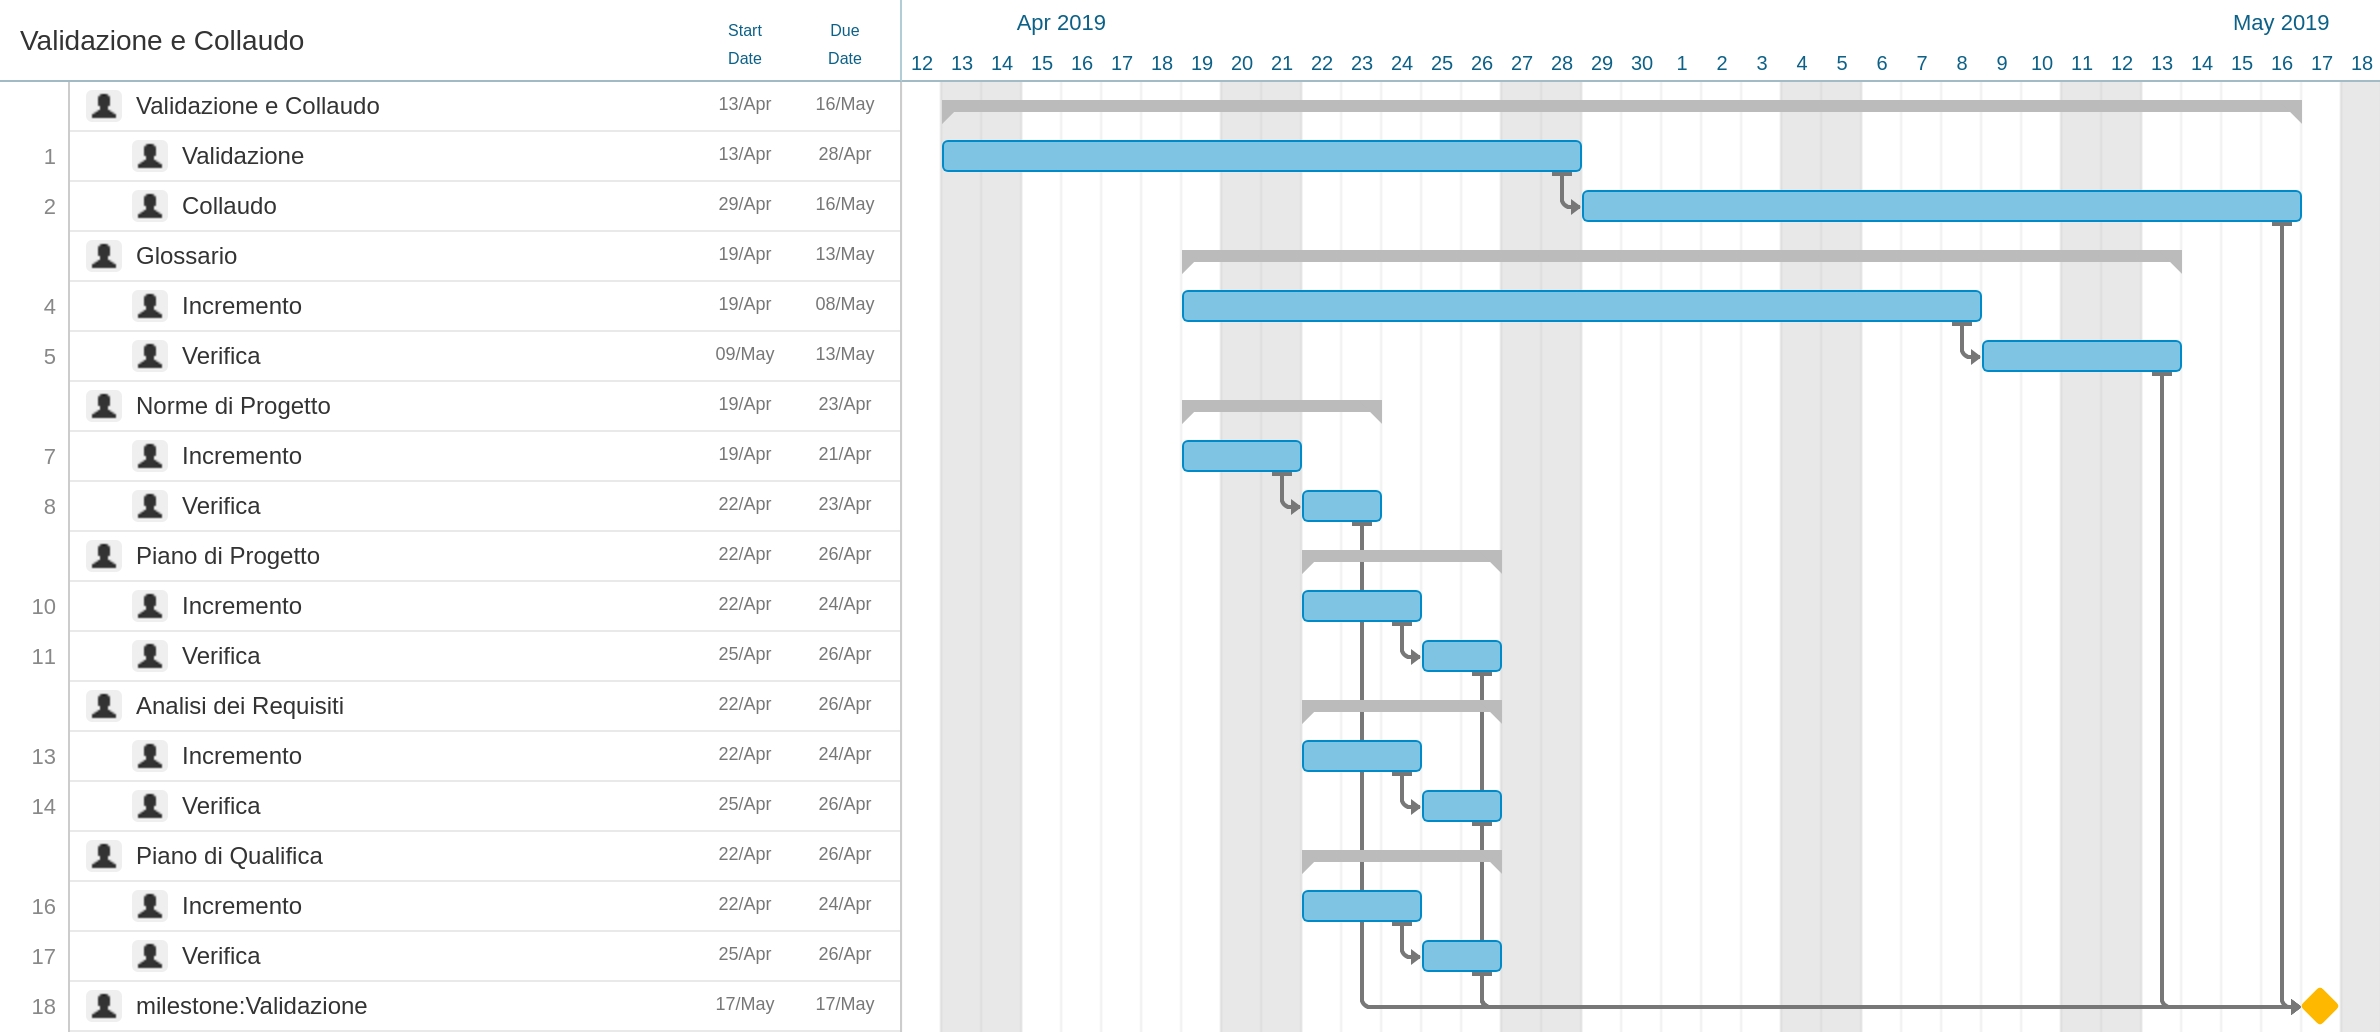
\includegraphics[scale=0.14]{./images/validazione_collaudo.jpg}
    \caption{\textit{Diagramma di}\glossario{Gantt}: Validazione e Collaudo }\label{}
\end{figure}